\documentclass[
  bibliography=totoc,     % Literatur im Inhaltsverzeichnis
  captions=tableheading,  % Tabellenüberschriften
  titlepage=firstiscover, % Titelseite ist Deckblatt
]{scrartcl}

% Paket float verbessern
\usepackage{scrhack}

% Warnung, falls nochmal kompiliert werden muss
\usepackage[aux]{rerunfilecheck}

% unverzichtbare Mathe-Befehle
\usepackage{amsmath}
% viele Mathe-Symbole
\usepackage{amssymb}
% Erweiterungen für amsmath
\usepackage{mathtools}

% Fonteinstellungen
\usepackage{fontspec}
% Latin Modern Fonts werden automatisch geladen
% Alternativ zum Beispiel:
%\setromanfont{Libertinus Serif}
%\setsansfont{Libertinus Sans}
%\setmonofont{Libertinus Mono}

% Wenn man andere Schriftarten gesetzt hat,
% sollte man das Seiten-Layout neu berechnen lassen
\recalctypearea{}

% deutsche Spracheinstellungen
\usepackage[ngerman]{babel}


\usepackage[
  math-style=ISO,    % ┐
  bold-style=ISO,    % │
  sans-style=italic, % │ ISO-Standard folgen
  nabla=upright,     % │
  partial=upright,   % │
  mathrm=sym,        % ┘
  warnings-off={           % ┐
    mathtools-colon,       % │ unnötige Warnungen ausschalten
    mathtools-overbracket, % │
  },                       % ┘
]{unicode-math}

% traditionelle Fonts für Mathematik
\setmathfont{Latin Modern Math}
% Alternativ zum Beispiel:
%\setmathfont{Libertinus Math}

\setmathfont{XITS Math}[range={scr, bfscr}]
\setmathfont{XITS Math}[range={cal, bfcal}, StylisticSet=1]

% Zahlen und Einheiten
\usepackage[
  locale=DE,                   % deutsche Einstellungen
  separate-uncertainty=true,   % immer Unsicherheit mit \pm
  per-mode=symbol-or-fraction, % / in inline math, fraction in display math
]{siunitx}

% chemische Formeln
\usepackage[
  version=4,
  math-greek=default, % ┐ mit unicode-math zusammenarbeiten
  text-greek=default, % ┘
]{mhchem}

% richtige Anführungszeichen
\usepackage[autostyle]{csquotes}

% schöne Brüche im Text
\usepackage{xfrac}

% Standardplatzierung für Floats einstellen
\usepackage{float}
\floatplacement{figure}{htbp}
\floatplacement{table}{htbp}

% Floats innerhalb einer Section halten
\usepackage[
  section, % Floats innerhalb der Section halten
  below,   % unterhalb der Section aber auf der selben Seite ist ok
]{placeins}

% Seite drehen für breite Tabellen: landscape Umgebung
\usepackage{pdflscape}

% Captions schöner machen.
\usepackage[
  labelfont=bf,        % Tabelle x: Abbildung y: ist jetzt fett
  font=small,          % Schrift etwas kleiner als Dokument
  width=0.9\textwidth, % maximale Breite einer Caption schmaler
]{caption}
% subfigure, subtable, subref
\usepackage{subcaption}

% Grafiken können eingebunden werden
\usepackage{graphicx}

% schöne Tabellen
\usepackage{tabularray}
\UseTblrLibrary{booktabs, siunitx}

% Verbesserungen am Schriftbild
\usepackage{microtype}

% Literaturverzeichnis
\usepackage[
  backend=biber,
]{biblatex}
% Quellendatenbank
\addbibresource{lit.bib}
\addbibresource{programme.bib}

% Hyperlinks im Dokument
\usepackage[
  german,
  unicode,        % Unicode in PDF-Attributen erlauben
  pdfusetitle,    % Titel, Autoren und Datum als PDF-Attribute
  pdfcreator={},  % ┐ PDF-Attribute säubern
  pdfproducer={}, % ┘
]{hyperref}
% erweiterte Bookmarks im PDF
\usepackage{bookmark}

% Trennung von Wörtern mit Strichen
\usepackage[shortcuts]{extdash}

\author{%
  Vincent Wirsdörfer\\%
  \href{mailto:vincent.wirsdoerfer@udo.edu}{authorA@udo.edu}%
  \and%
  Joris Daus\\%
  \href{mailto:joris.daus@udo.edu}{authorB@udo.edu}%
}
\publishers{TU Dortmund – Fakultät Physik}


\begin{document}
\section{Diskussion}
\label{sec:Diskussion}

Die Sichtung der Messdaten vermittelt auf den ersten Blick eine gelungene Durchführung. Die Intensitätsabnahme in der 
Nähe des Brewsterwinkels ist bei dem parallel polarisiertem Licht eindeutig zu erkennen. Es ist allerdings zu erwähnen, 
dass die gemessene Intensität nicht wie durch die Gleichung vorausgesagt auf null abfällt, sondern mehr einem Minimum 
gleicht. Aus diesem Grund ist das Minimum kein Peak, sondern mehr ein Bereich. Weil das Minimum bestimmt wird, indem 
der kleinste Wert der Messdaten genommen wird, ist die Streuung des minimalen Winkels nicht berücksichtigt.

\noindent Wie in der Auswertung bereits erwähnt, ist der Brechungsindex stark von dem Winkel abhängig, was theoretisch nicht der 
Fall sein sollte. Außerdem muss ein Korrekturfaktor eingeführt werden, damit die Messdaten überhaupt gefittet werden 
können. All dies spricht nicht für eine Reibungsfreie Durchführung. \\
\noindent Nichtsdestotrotz sind die Brechungsindizes alle dicht beieinander: 

\begin{align*}
    n_\parallel &= \num{3.64 \pm 0.06}\\
    n_\bot      &= \num{3.48 \pm 0.12}\\
    n_\text{tan} &=\num{3.49\pm0.11}
\end{align*}

\noindent Der Literaturwert des Brechungsindex von Silizium bei einer Wellenlänge von \qty{633}{\nano\meter} liegt bei 
$n_\text{Lit}=\num{3.88}$ \cite{Brechungsindex_SI}. So wird die Abweichung vom Literaturwert auf folgende Werte bestimmt:

\begin{align*}
    \Delta n_\parallel &= \qty{6.3  \pm 1.5}{\percent}\\
    \Delta n_\bot      &= \qty{10.4 \pm 3.0}{\percent}\\
    \Delta n_\text{tan} &=\qty{10.1 \pm 3.0}{\percent}
\end{align*}

\noindent Aus dem Literaturwert des Brechungsindexes kann über $\alpha_\text{Lit}=\arctan{(n_\text{Lit})}$ der theoretische 
Brewsterwinkel bestimmt werden. So liegen der gemessene und der theoretische Brewsterwinkel bei

\begin{align*}
    \alpha_\text{Mess} &= \qty{74}{\degree} \\
    \alpha_\text{Lit}  &= \qty{75.55}{\degree} \\
\end{align*}

\noindent Die daraus folgende Abweichung des gemessenen Brewsterwinkels zum berechneten Brewsterwinkel beträgt 

\begin{align*}
    \Delta \alpha_\text{Mess} &= \qty{2.0\pm0.7}{\percent}.
\end{align*}

\noindent Zusätzliche mögliche Gründe, zu den bereits erwähnten werden nun benannt.\\
\noindent Trotz der kleinen Schrittweite der Winkel kann es aufgrund von statistischen Fehlern dazu kommen, dass im Bereich 
des Brewsterwinkels gemessene Intensitäten zu hoch oder zu niedrig konstatiert werden. Dies hat als direkte Folge, dass der 
Brewsterwinkel sich um \qty{1}{\degree} verschiebt. Dies kann hier der Fall gewesen sein.\\
\noindent Des Weiteren emittiert der He-Ne Laser nicht nur eine Wellenlänge, sondern auch ein Spektrum aus mehreren einzelnen 
Wellenlängen. Dies kann die gemessene Intensität höher wirken lassen, als sie ist.\\
\noindent Das analoge Strommessgerät zeigt keine konstanten Werte an, sondern die Werte schwanken viel mehr in einem Bereich. 
Genaue Werte abzulesen ist so nicht möglich. Externe Lichteinflüsse aus dem Umgebungslicht stören die Messung. Als Beispiel 
sorgt eine Öffnung der Tür für Einfall von Licht. Außerdem kann für große Winkel der Laser direkt in die Photodiode strahlen, 
ohne am Spiegel reflektiert worden zu sein. Aus diesem Grund wird nur bis \qty{87}{\degree} gemessen.


%laser emmitiert auch andere Spektren -> Messung nicht sensibel über differenzierte Wellenlängen sondern über alle zusammen
%Spektrum des Lasers vermatscht messung


\section{Anhang}

\begin{figure}[H]
    \centering
    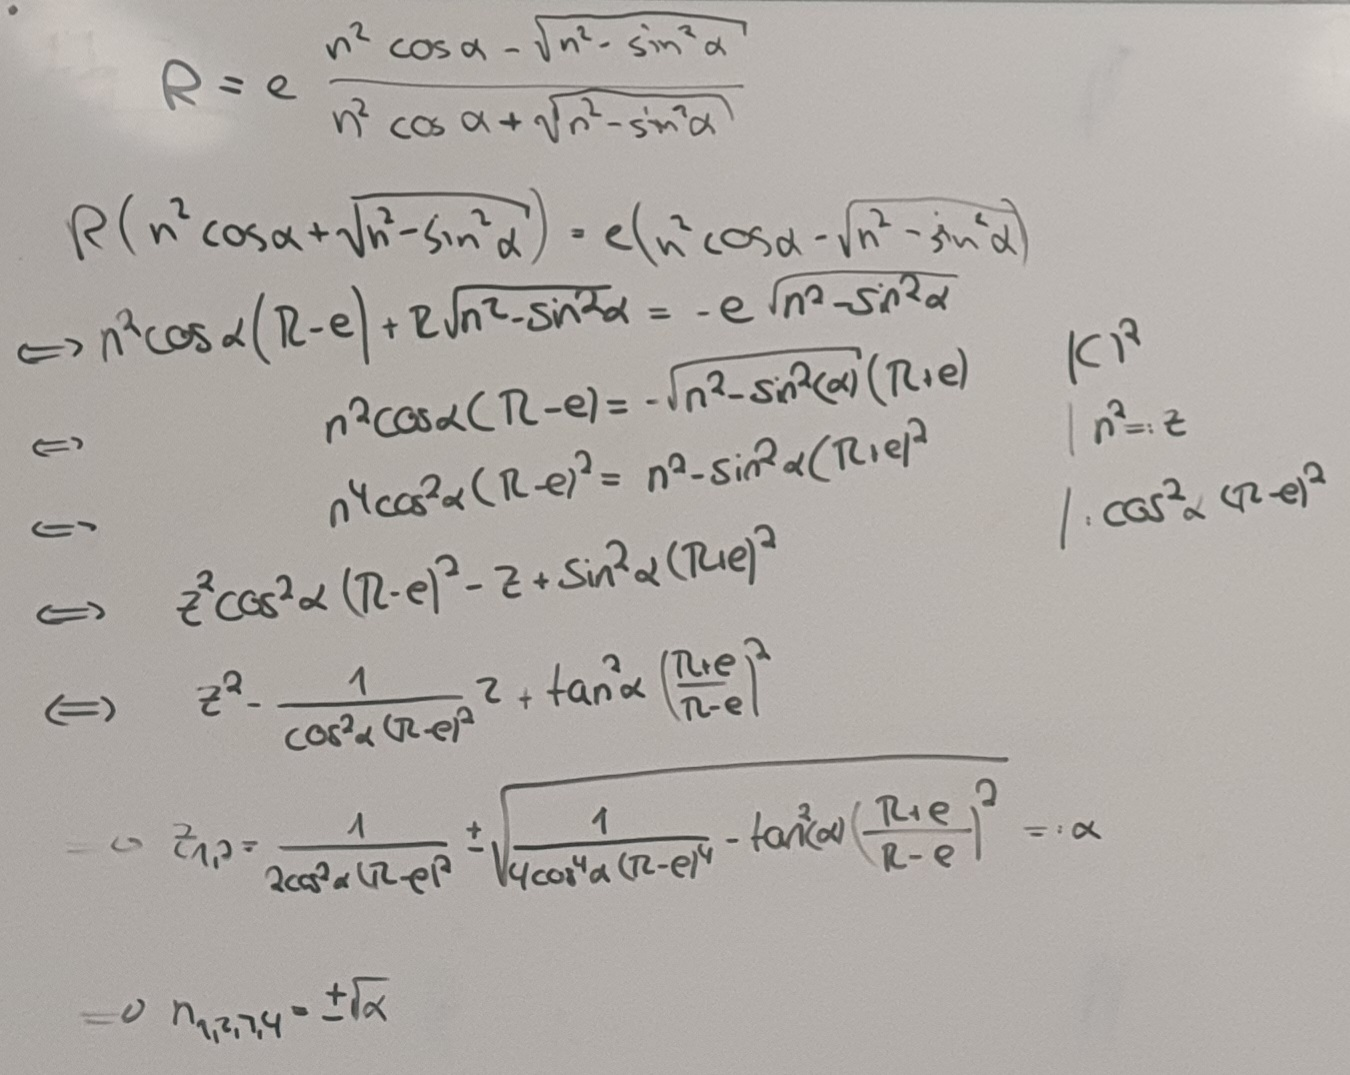
\includegraphics[width=0.9\textwidth]{Gleichung21.jpg}
    \caption{Umstellung der Gleichung der parallelen Reflexion.}
\end{figure}

\begin{figure}[H]
    \centering
    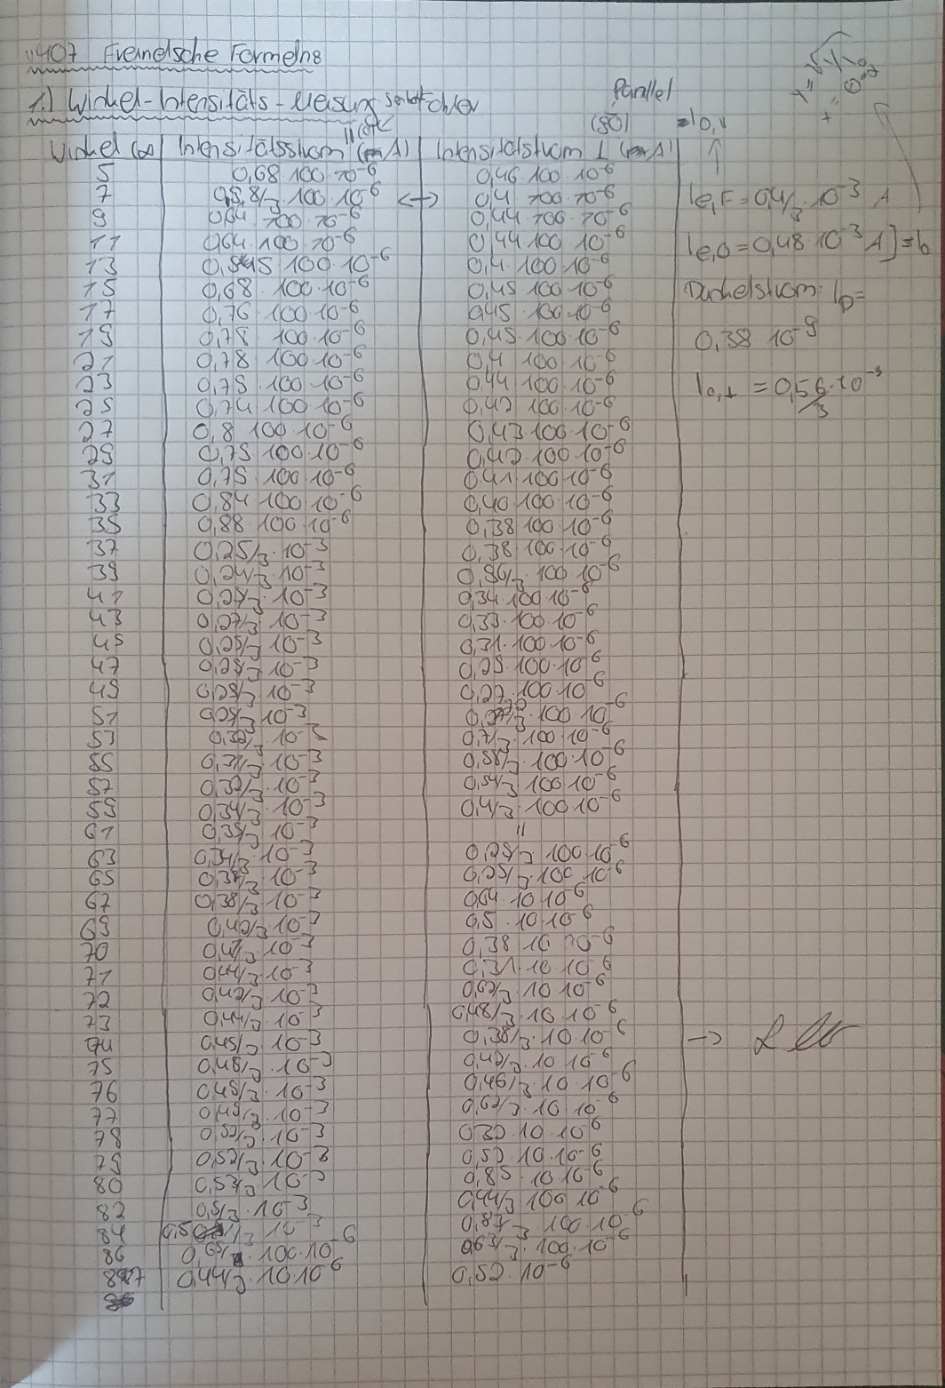
\includegraphics[width=0.9\textwidth]{Laborbuch.jpg}
    \caption{Foto der Messdaten aus dem Laborbuch.}
\end{figure}




\end{document}
